\section{Praktikum}

Berikut ini adalah board FPGA yang akan kita gunakan dalam praktikum ini.

\begin{figure}[H]
{\centering
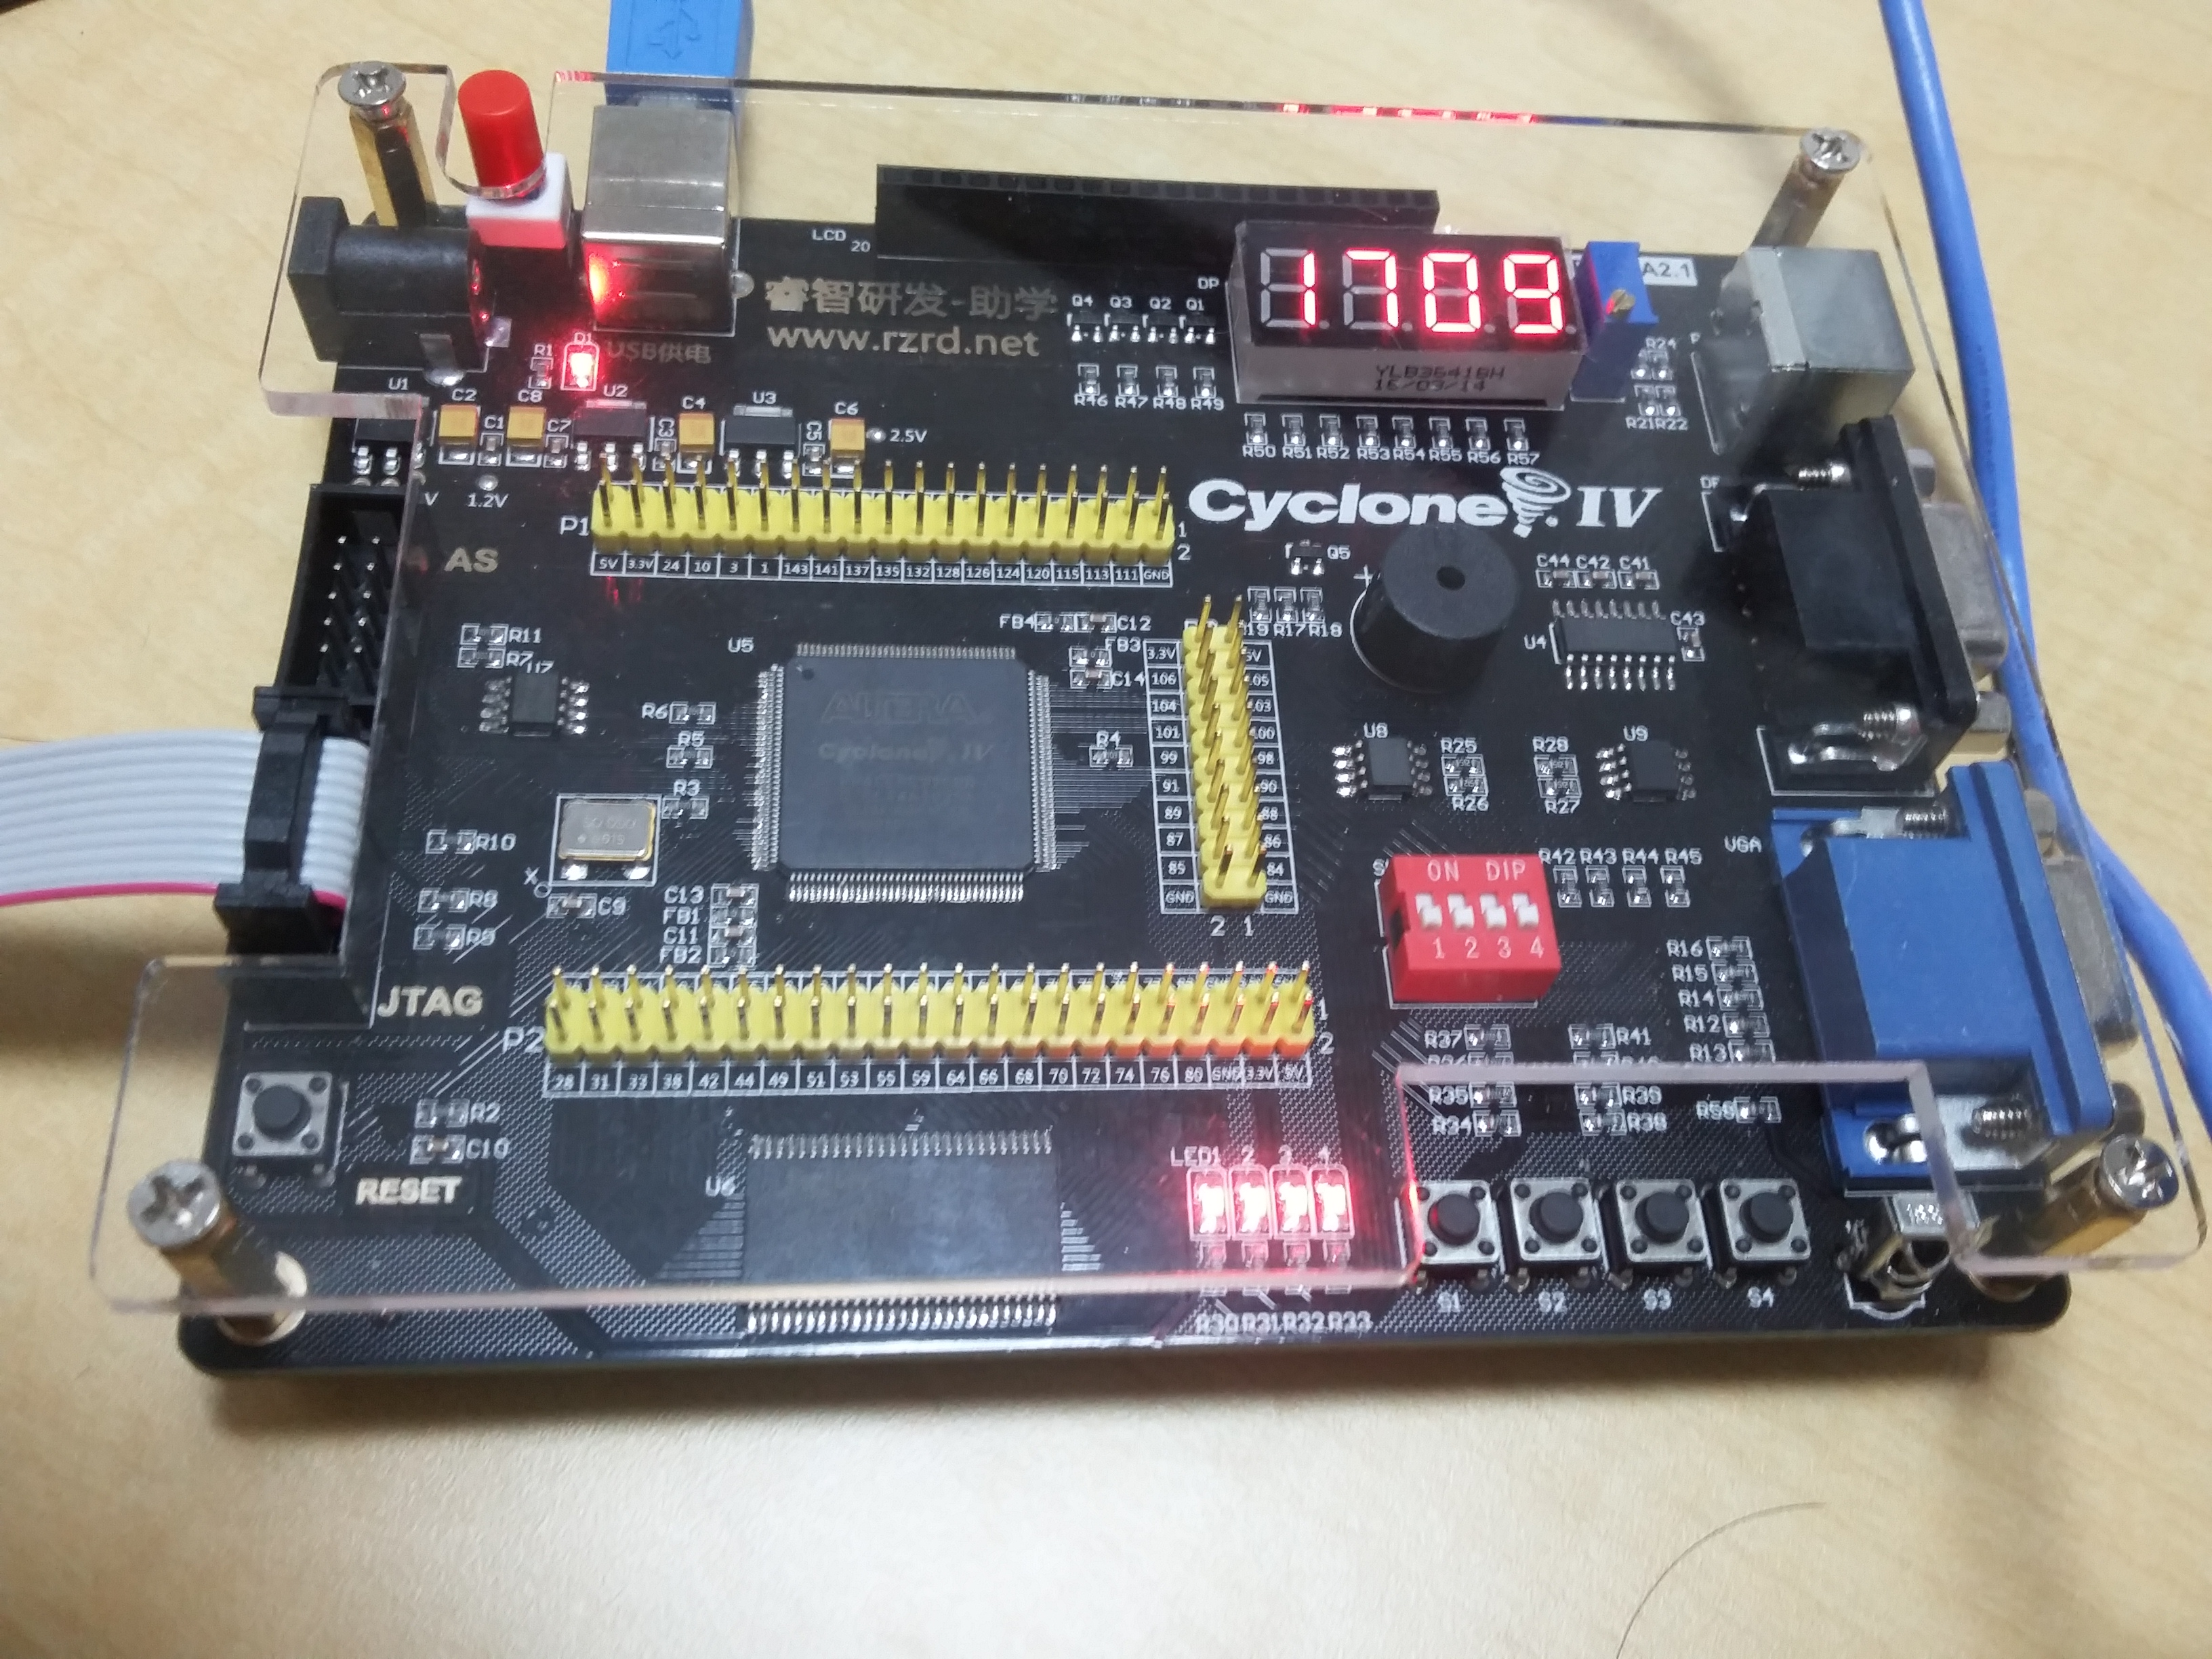
\includegraphics[width=0.5\textwidth]{images/foto_FPGA_v1.jpg}
\par}
\caption{FPGA Board Versi A}
\end{figure}

{\color{red}Perlu gambar FPGA yang kedua dan informasi PIN untuk board kedua.}

Berikut ini adalah pedoman umum yang akan kita lakukan pada praktikum ini.

\begin{itemize}

\item Buat proyek Quartus Prime baru, misalkan dengan nama \textbf{Modul5\_Kelompok\_XX}.
di dalam direktori dengan nama yang sama. \textit{Hindari penggunaan
spasi dalam nama proyek}.

\item Langkah untuk menambahkan file skematik baru dapat dilakukan sesuai dengan langkah yang
dijelaskan pada bagian \ref{subsec:skematik}. Penambahan file Verilog
juga dapat dilakukan dengan cara yang mirip.

\item Sebelum melakukan kompilasi desain (skematik atau Verilog)
pastikan bahwa desain tersebut telah dibuat menjadi top-level entity
\footnote{Top-level entity memiliki peran yang sama
dengan fungsi \texttt{main} pada bahasa C/C++}
melalui menu \textbf{Project $\rightarrow$ Set as Top-Level Entity} atau
keyboard shortcut \textbf{Ctrl+Shift+J}.

\item Lakukan kompilasi setelah desain selesai dibuat.

\item Lakukan PIN assignment. Pastikan bahwa semua port yang akan digunakan
telah diberikan PIN yang sesuai.

\item Lakukan kompilasi sekali lagi.

\item Download desain yang telah dibuat ke FPGA dan verifikasi apakah telah berjalan
sesuai dengan yang diharapkan.
\end{itemize}

Langkah-langkah tersebut akan diilustrasikan pada eksperimen dengan LED.
